\documentclass[12pt,compress]{beamer}
\usepackage{ifthen,verbatim}

\title{\mbox{Latest Submission to SiStripElectronProducer} \\ and the \\ State of Pixelless Electron-Finding}
\author{Jim Pivarski}
\institute{Cornell University}
\date{4 August, 2006}

\setbeamertemplate{navigation symbols}{}
\setbeamertemplate{headline}{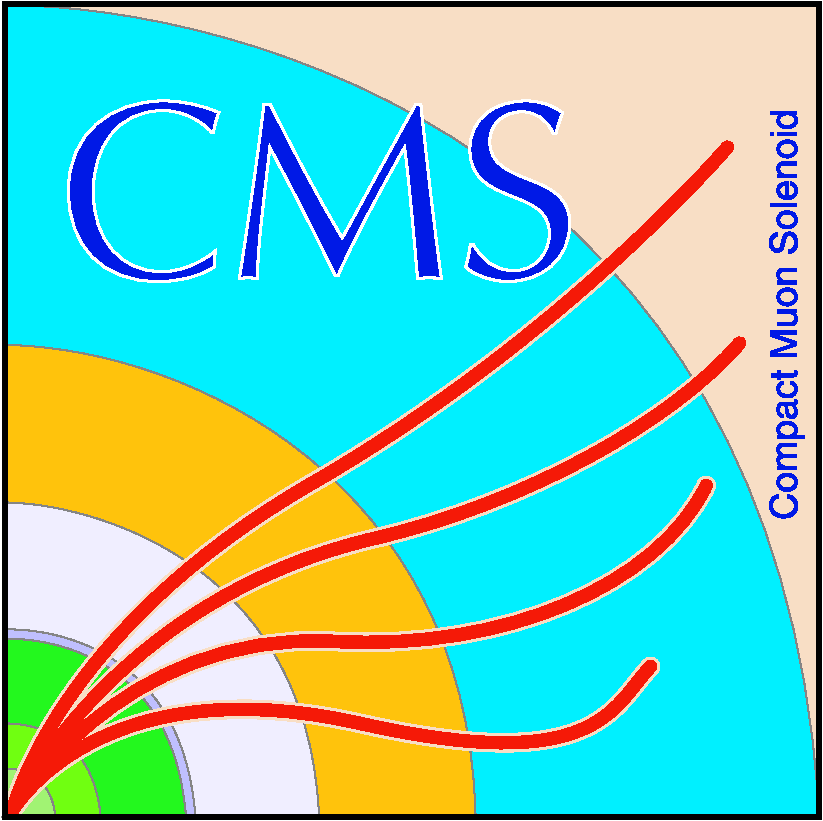
\includegraphics[height=1 cm]{cmslogo} \hfill
\begin{minipage}{8 cm}
\vspace{-0.75 cm} \small
\begin{center}
\ifthenelse{\equal{\insertpagenumber}{0}}{}{\insertsection\ (\insertpagenumber/\pageref{numpages})}
\end{center}
\end{minipage} \hfill 
\includegraphics[height=1 cm]{lepplogo}}

\xdefinecolor{verylightgray}{rgb}{0.95,0.95,0.95}
\beamertemplateshadingbackground{verylightgray}{white}

\begin{document}
\addtocounter{page}{-1}
\frame{\titlepage}
\section*{SiStripElectronProducer --- Jim Pivarski}

\begin{frame}
\frametitle{Current Status:}
\begin{itemize}\setlength{\itemsep}{0.25 cm}
\item Complete structure for pixelless electron-finding is in place (in August 4's nightly and maybe {\tt CMSSW\_0\_9\_0\_pre3})
\begin{itemize}
\item Match SiStrip hits to SuperCluster
\item Drop hits with bad $\chi^2$
\item Seed track-fitting
\item Fit tracks
\item Associate fitted tracks with electron seeds
\item Make high-level reco::Electron objects
\end{itemize}

\item Tracking efficiency problem mostly solved (3\% $\longrightarrow$ 75\%)

\item Hit-matching algorithm (the interesting part) remains simplistic
\end{itemize}
\end{frame}

\begin{frame}
\frametitle{Structure of the Latest Code}
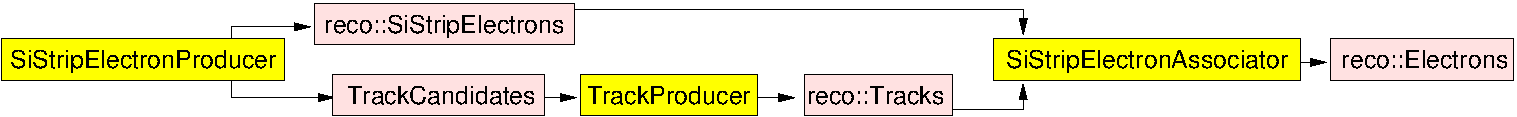
\includegraphics[width=\linewidth]{SiStripElectron_path}

\vfill
\begin{minipage}{\linewidth}
\small
\begin{description}
\item[SiStripElectronProducer] matches SiStrip hits to SuperClusters,
drops hits with bad $\chi^2$, creates SiStripElectrons and
TrackCandidates
\item[reco::SiStripElectron] is a reco::Candidate containing references
to SuperCluster and hits, as well as diagnostic information about the
hit-matching
\item[SiStripElectronAssociator] associates reconstructed Tracks with
the electrons that seeded them, outputs high-level reco::Electrons
\end{description}
\end{minipage}
\end{frame}

\begin{frame}
\frametitle{Tracking Efficiency}

\begin{itemize}
\item Sorting hits radially brought efficiency up from 3\% to 75\%
\item Dropping hits with bad $\chi^2$ should also help (untested)
\end{itemize}

\begin{center}
\begin{tabular}{p{0.45\linewidth} p{0.45\linewidth}}
\begin{minipage}{\linewidth}
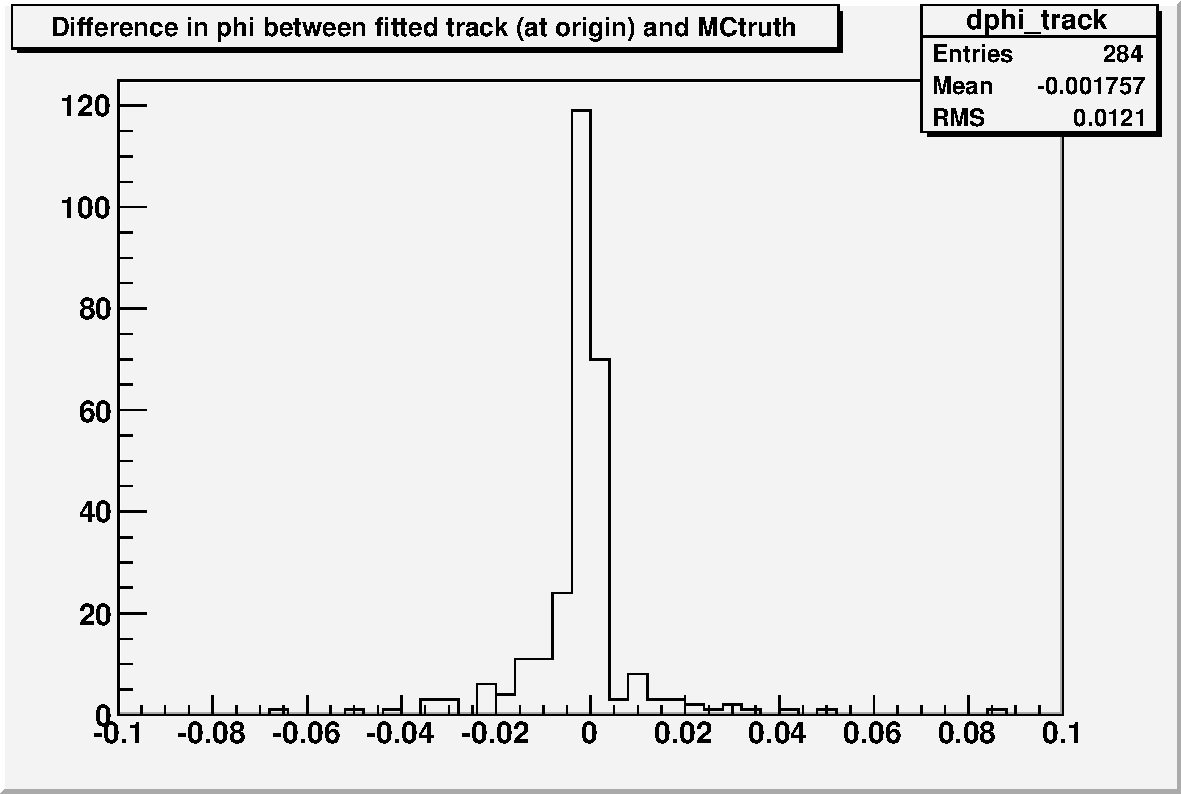
\includegraphics[width=\linewidth, height=2.5 cm]{dphi_track}
\end{minipage} &
\begin{minipage}{\linewidth}
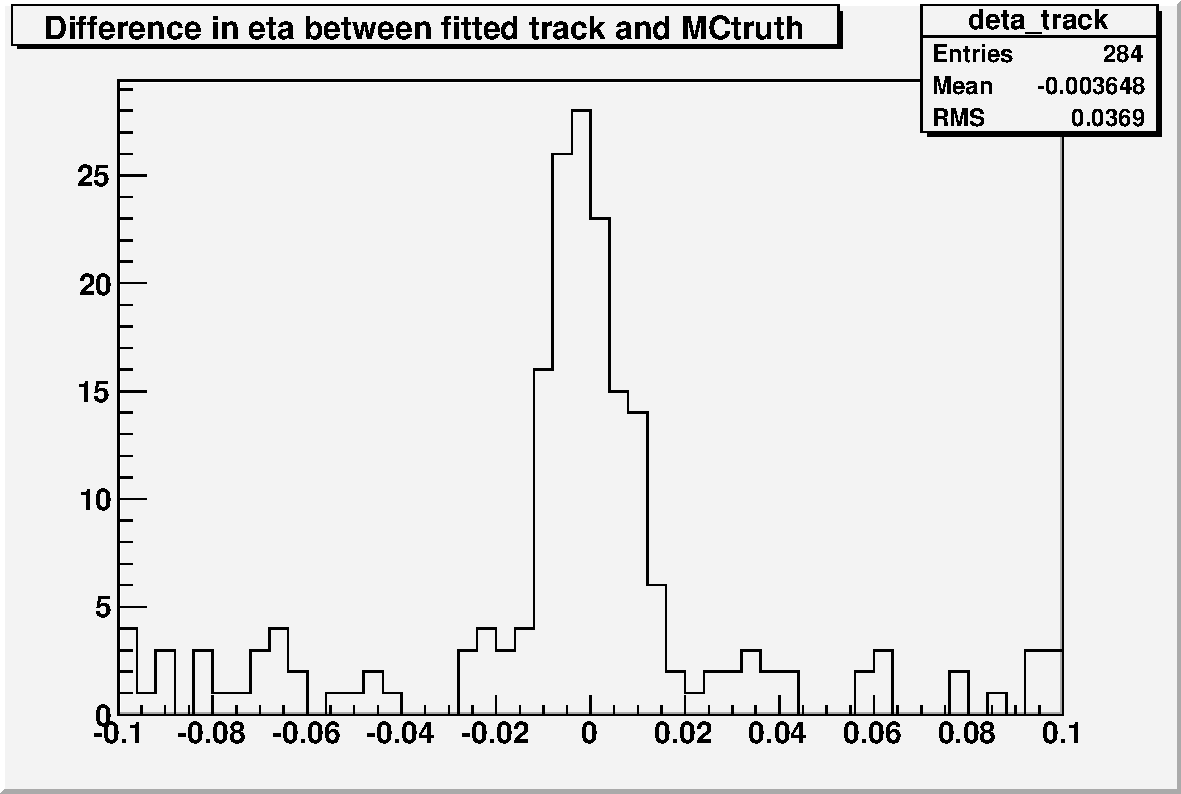
\includegraphics[width=\linewidth, height=2.5 cm]{deta_track}
\end{minipage} \\
& \\
\begin{minipage}{\linewidth}
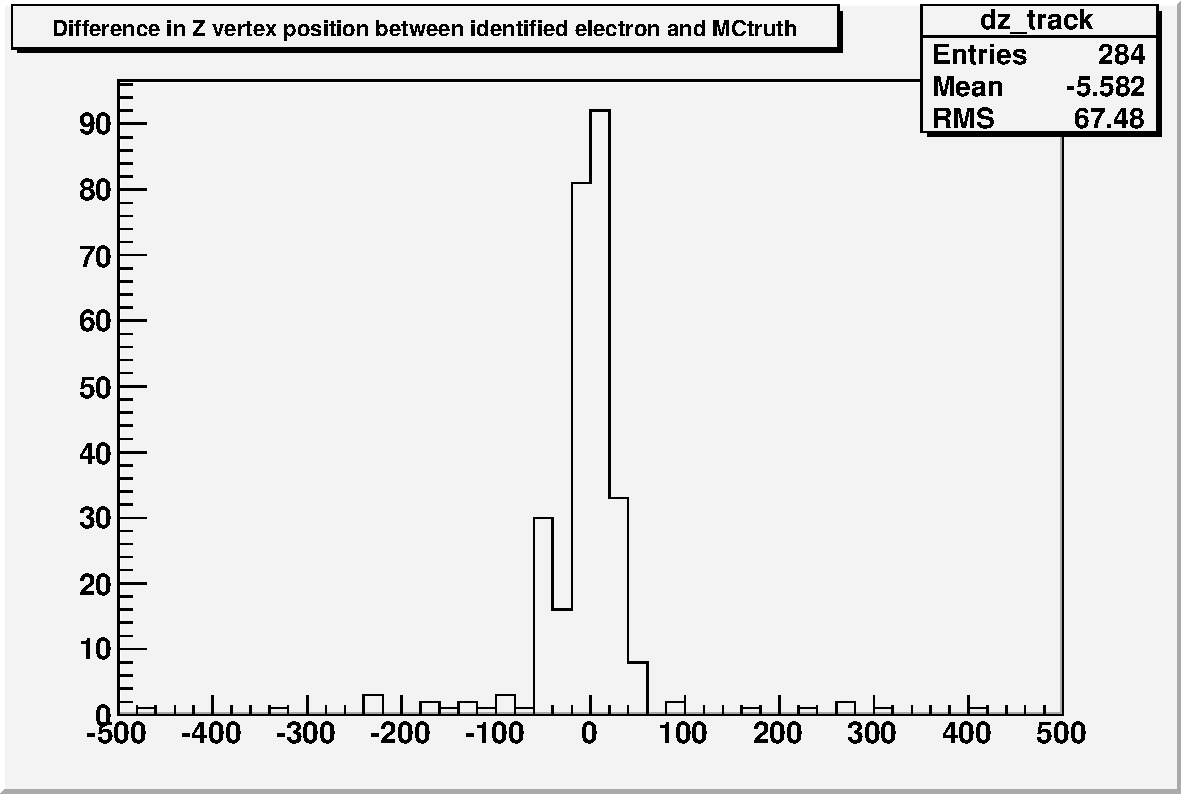
\includegraphics[width=\linewidth, height=2.5 cm]{dz_track}
\end{minipage} &
\begin{minipage}{\linewidth}
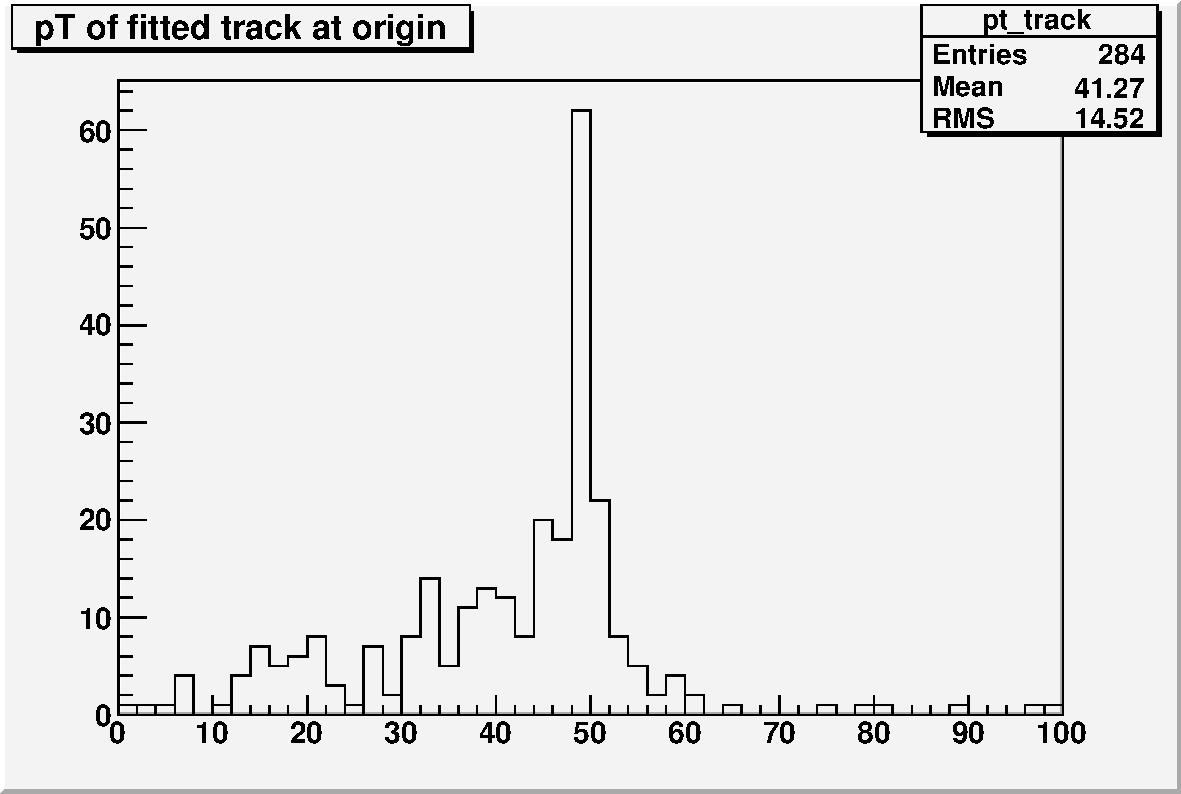
\includegraphics[width=\linewidth, height=2.5 cm]{pt_track}
\end{minipage}
\end{tabular}
\end{center}
\end{frame}

\begin{frame}
\frametitle{Hit-Matching is still the Band Algorithm}

\begin{center}
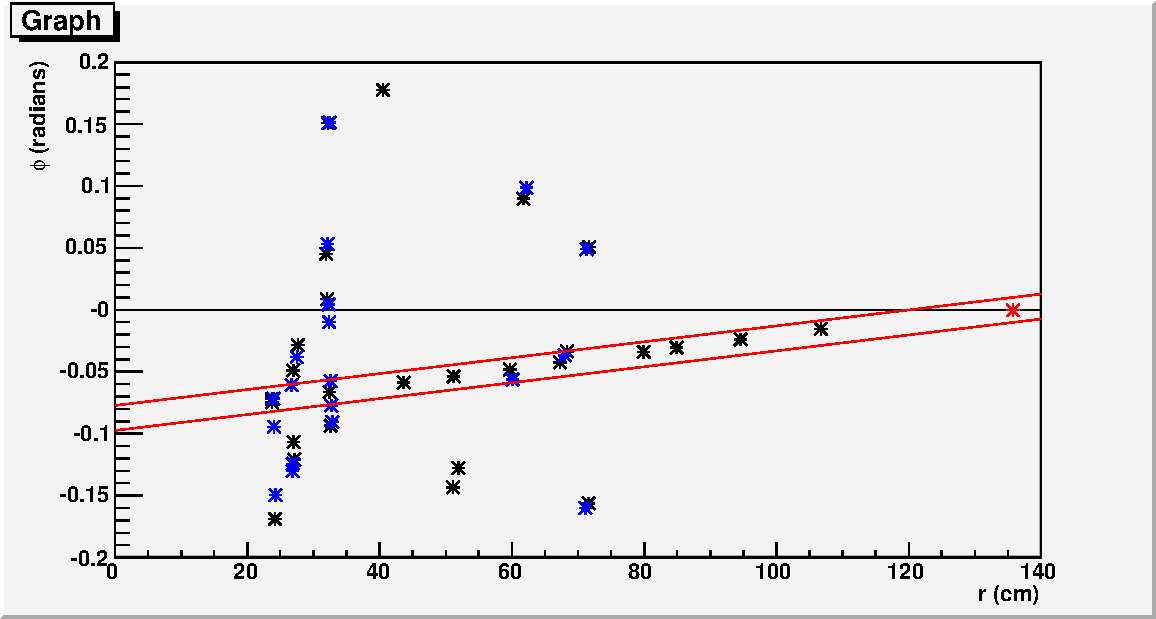
\includegraphics[width=\linewidth]{event_display_banded}
\end{center}

\vspace{-0.25 cm}
\ldots though we now throw out hits with $\chi^2_i > 10$
\end{frame}

\begin{frame}
\frametitle{The look of things to come}

\begin{itemize}
\item I'm leaving Cornell (going to Texas A\&M to do $\tau^\pm$ reconstruction)
\item Jean is taking over this project
\begin{itemize}
\item He's been involved all along
\item Already getting data from ElectronAnalyzer to FWLite
\item He will focus on hit-matching algorithms (the physics)
\item He'd be giving here, giving this talk, if it were not for a sudden emergency
\end{itemize}
\item Expect revisions in SiStripElectronProducer's choice of hits (to
improve electron identification and tracking efficiency), but only
bug-fixes in the rest of the infrastructure
\end{itemize}
\label{numpages}
\end{frame}

\end{document}
